%% The first command in your LaTeX source must be the \documentclass command.
\documentclass[acmtog]{acmart}
\usepackage[english,ngerman]{babel}
\usepackage[utf8]{inputenc} 

%% \BibTeX command to typeset BibTeX logo in the docs
\AtBeginDocument{%
  \providecommand\BibTeX{{%
    \normalfont B\kern-0.5em{\scshape i\kern-0.25em b}\kern-0.8em\TeX}}}
    
\copyrightyear{2024}
\acmYear{2024}
\citestyle{acmauthoryear}

\usepackage[figurename=Fig.]{caption}
\usepackage{csquotes}
\setcopyright{none}
\makeatletter
\renewcommand{\fnum@figure}{Abb. \thefigure}
\makeatother
\addto\captionsngerman{\renewcommand{\figurename}{Abb.}}
\settopmatter{printacmref=false} % Removes citation information below abstract
\renewcommand\footnotetextcopyrightpermission[1]{} % removes footnote with conference information in first column

\usepackage{minted}

%%
%% end of the preamble, start of the body of the document source.
\begin{document}

%%
%% The "title" command has an optional parameter,
%% allowing the author to define a "short title" to be used in page headers.
\title{Enterprise Architektur-Muster}

%%
%% The "author" command and its associated commands are used to define
%% the authors and their affiliations.
%% Of note is the shared affiliation of the first two authors, and the
%% "authornote" and "authornotemark" commands
%% used to denote shared contribution to the research.
\author{Julian Bruder}
\authornote{Alle Studierenden trugen zu gleichen Teilen zu dieser Arbeit bei.}
\author{Abdellah Filali}
\authornotemark[1]
\author{Luca Franke}
\authornotemark[1]
\affiliation{%
  \institution{Hochschule für Technik, Wirtschaft und Kultur Leipzig (HTWK Leipzig)}
  \streetaddress{Karl-Liebknecht-Str. 132}
  \city{Leipzig}
  \country{Deutschland}
  \postcode{04277}
}
%%
%% By default, the full list of authors will be used in the page
%% headers. Often, this list is too long, and will overlap
%% other information printed in the page headers. This command allows
%% the author to define a more concise list
%% of authors' names for this purpose.
\renewcommand{\shortauthors}{Bruder, Filali, Franke}

%%
%% The abstract is a short summary of the work to be presented in the
%% article.
\begin{abstract}
Blah abstrakt\ldots
\end{abstract}

\maketitle

\section{Einleitung}
% (Beschreibung von Kontext, Problemen, Anforderungen und Zielen)
Mit E-Commerce-Beispiel motivieren

\section{Grundlagen von Enterprise-Architekturen}
Verteilte Systeme \ldots

Architekturen \ldots

Komponenten \ldots

\ldots


\section{Klassische Enterprise-Architekturen}

\subsection{Service-oriented}
Die Service-oriented Achitectur (SOA) basiert sich auf die Verwendung von Services. 
Ein Service kapselt ein Dienst, das über eine definierte Schnittstelle interagiert \cite{soa}[S. 3]. 
Dieses kann aus einer Reihe von Komponenten bestehen, die gemeinsam eine 
bestimmte Funktionalität bereitstellen. Der Zugriff auf den Service erfolgt über das Netzwerk,
typischerweise mithilfe eines Namens oder eines Locators \cite{soa2}[S. 3].

Betrachten wir im Folgenden die Hauptbestandteile einer SOA:
\begin{itemize}
  \item Service Provider: Liefert ein bestimmtes Dienst
  \item Service Broker: Dienst, das die Komunikation zwischen Service Requester und Service Broker reguliert und koordiniert.
  \item Service Request: Nutzt einen bereitgestelten Dienst 
\end{itemize}

Der Sevice Broker kann als ein Vermittler interpretiert werden. In der SOA ein Sevice 
Provider sendet den Service Broker Informationen (publisch), die den Service Requester helfen den Dienst zu verwenden.
Der Sevice Provieder sendet eine Beschreibung den angeförderten Diest (publish) und 
Der Service Broker liefert den am besten passenden Dienst, indem er die Provider-ID 
des entsprechenden Dienstanbieters mitteilt.Schließlich nehmen sowohl der Service Provider 
als auch der Service Requester direktr miteinander Kontakt auf, und die Eigentümer der 
jeweiligen Dienste führen diese gemeinsam aus (bind) . \cite{soa2}[S. 4]
Die Abbildung ~\ref{fig:soa} fasst diese Beziehung zusammen.
\begin{figure}[h]
  \centering
  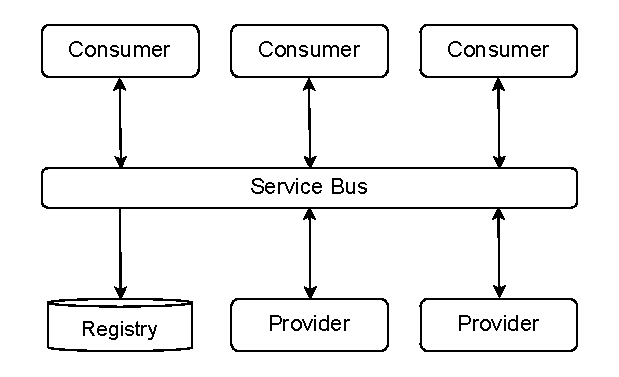
\includegraphics[width=0.85\linewidth]{images/soa/soa.pdf}
  \caption{Aufbau Service-oriented Architecture}
  \label{fig:soa}
\end{figure}

Die lose Kopplung von den Services ermöglicht die Änderung von diesen ohne 
großen Einflüsse auf das gesamten System, was die Agilität fördert.
Außerdem jedes Service kann von kleinen Agile-Teams entwicklt werden 
was die maximale Skalierung ermöglicht.

Insgesamt weist die Service-oriented Architecture also eine sehr hohe Agilität auf.

Betrachten wir erneut das E-Commerce-Beispiel aus der Einleitung.
Dafür definieren wir drei Arten von Services:
\begin{itemize}
  \item \texttt{OrderService}: Ein Dienst, das genau dann angesprochen wird, wenn eine neue Bestellung aufgegeben wird
  \item \texttt{PaymentService}: Ein Dienst, das genau dann angesprochen wird, wenn der Bezahlvorgang gestartet wird
  \item \texttt{ShipmentService}: Ein Dienst, das genau dann angeprochen wird, wenn der Bezahlvorgang erfolgreich war und der Versandvorgang gestart wird
\end{itemize}

\begin{figure}[!h]
  \centering
  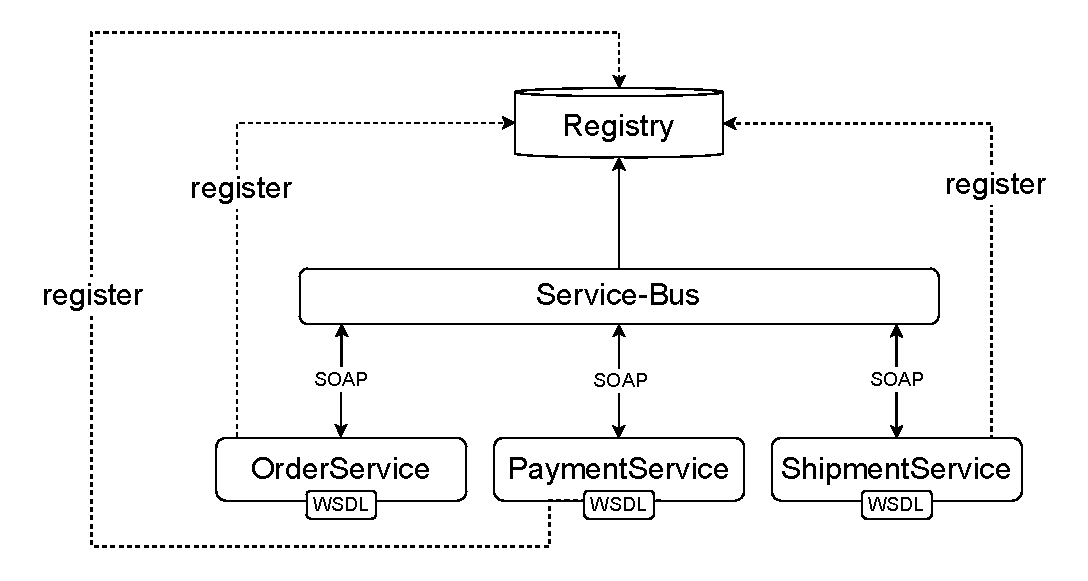
\includegraphics[width=0.8\linewidth]{images/soa/soa-example.pdf}
  \caption{E-Commerce-Beispiel mit Service-oriented Architecture}
  \label{fig:soaecommerce}
\end{figure}

Wie Abbildung \ref{fig:soaecommerce} zeigt, die Dienste\texttt{ShipmentService} 
und \texttt{PaymentService} werden als externe Dienste betrachtet, die ihre Informationen 
(Name, Bescheibung des Dienstes und Endpoint) bei dem Broker veröffentlichen.
Der \texttt{OrderService} ist ein interner Dienst, der die beiden externen Dienste
 verwendet. Dies erfolgt durch Anfragen an den Broker, der die entsprechenden Endpoints
 der Dienste ermittelt, sodass der \texttt{OrderService} über HTTP-Requests auf die benötigten 
 Dienste zugreifen kann.

Das Beispiel zeigt, wie die Service-oriented Architecture die Agilität fördern kann.
Externe Dienste können ohne große Anpassungen integriert werden und in internen 
Dienste kombiniert und verwendet werden. Neue Entwickler können an einzelnen Diensten arbeiten, 
ohne das gesamte System verstehen zu müssen, da die Dienste über definierte 
Schnittstellen miteinander kommunizieren.


Die vollständige Implementierung des E-Commerce-Beispiels ist bei GitHub \footnote{https://github.com/Beleg-6-EAP/demo-soa-ecommerce} zu finden.



\section{Moderne Enterprise-Architekturen}

\subsection{Event-Driven Architecture}
Die Event-Driven Architecture wählt als Basis einen anderen Ausgangspunkt als die bisherigen Architekturmuster.
Während bei letzteren Komponenten Dienste bereitstellen, welche von anderen Komponenten explizit genutzt werden,
verhalten sich Dienst-bereitstellende Komponenten in der Event-Driven Architecture reaktiv,
werden also implizit von Dienst-konsumierenden Komponenten genutzt \cite{garlanShawImplizit}.
Ein System reagiert somit asynchron auf Zustandsänderungen, also Ereignisse in diesem System \cite{eda}.
Die in dieser Architektur minimalen Einheiten, welche Informationen einer Zustandsänderung kapseln, werden \textit{Events} genannt.
Die Idee der impliziten Behandlung von Ereignissen ist nicht neu und taucht erstmals 1994 im von Garlan und Shaw publizierten Papier
\textit{\enquote{An introduction to Software Architecture}} auf.

Betrachten wir im Folgenden die Basis-Bestandteile der Event-Driven Architecture:
\begin{itemize}
  \item Ereignis (englisch \textit{Event}): Kapselt Information einer Zustandsänderung eines Systems
  \item Produzent (englisch \textit{Producer}): Komponente, die Event erzeugt
  \item Herausgeber (englisch \textit{Publisher}): Komponente, die, von Produzenten erzeugte, Events publiziert
  \item Konsument (englisch \textit{Consumer}): Komponente, die auf publizierte Events reagiert
  \item Vermittler (englisch \textit{Mediator}): Komponente zwischen Produzenten und Konsumenten - filtert Events und verteilt diese auf Konsumenten
  \item Event-Bus: Oft auch \textit{Event-Broker} genannt - bietet die Infrastruktur für die Gesamtheit der Vermittler
\end{itemize}
Abstrakt kann ein Event als Vertrag zwischen Produzenten und Konsumenten am Event-Bus betrachtet werden.
Der Konsument nutzt die Spezifikation des Events am Bus, der Produzent implementiert jene Spezifikation.
Abbildung \ref{fig:eda} stellt diesen Vertrag dar.

\begin{figure}[!h]
  \centering
  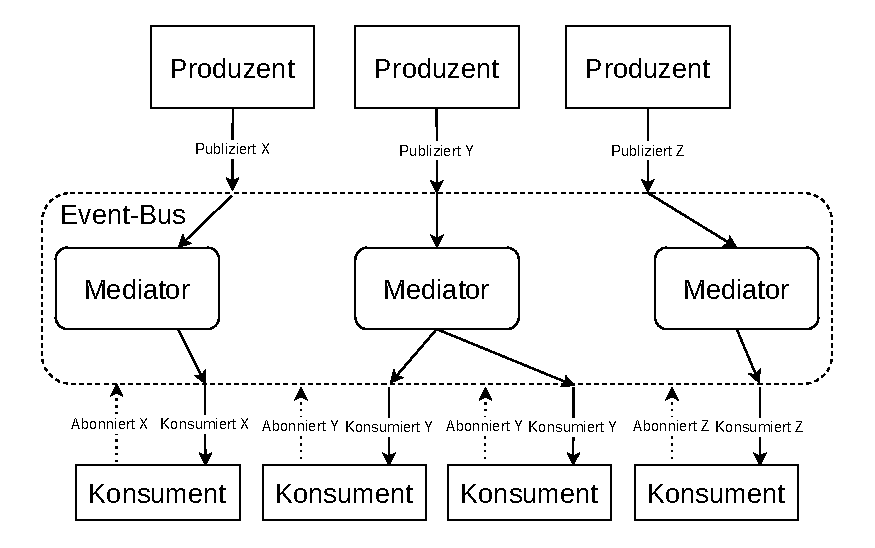
\includegraphics[width=\linewidth]{images/eda/eda.drawio}
  \caption{Vertrag zwischen Produzenten und Konsumenten am Event-Bus}
  \label{fig:eda}
\end{figure}

Durch den Vertrag weisen die Events am Event-Bus starke Kohäsion und somit lose Kopplung auf.
Diese lose Kopplung minimiert nicht nur kaskadierende Fehler, sondern ermöglicht agilen Entwickler-Teams durch klar abgegrenzte Features einfach definierbare Iterationen
- eine Menge von Events, deren Erzeugung und Konsumierung.

Weiter sind Events oft nah an dem, was Ereignisse in realen Prozessen sind, also domain-driven.
Gebündelt ermöglichen obige Punkte die kontinuierliche Auslieferung von Software in kurzen Intervallen.

Außerdem garantiert die asynchrone Behandlung von Ereignissen zusammen mit der loosen Kopplung maximale Skalierung.
Daher sind Event-Driven Architekturen besonders für datenintensive Echtzeit-Anwendungen wie IoT (Internet of Things) und Analytics geeignet \cite{iotEda}.

Betrachten wir erneut das E-Commerce-Beispiel aus der Einleitung.
Dafür definieren wir drei Arten von Events:
\begin{itemize}
  \item \texttt{OrderCreated}: Ein Event, das genau dann erzeugt wird, wenn eine neue Bestellung aufgegeben wird
  \item \texttt{PaymentProcessed}: Ein Event, das genau dann erzeugt wird, wenn der Bezahlvorgang abgeschlossen wird
  \item \texttt{ShipmentInitiated}: Ein Event, das genau dann erzeugt wird, wenn die Bestellung versandt wird
\end{itemize}

Weiter teilen wir die Funktionalität ähnlich wie bei der Microservice-Architektur in die drei verschiedenen Dienste \texttt{OrderService}, \texttt{PaymentService} und \texttt{ShipmentService} auf.

\begin{figure}[!h]
  \centering
  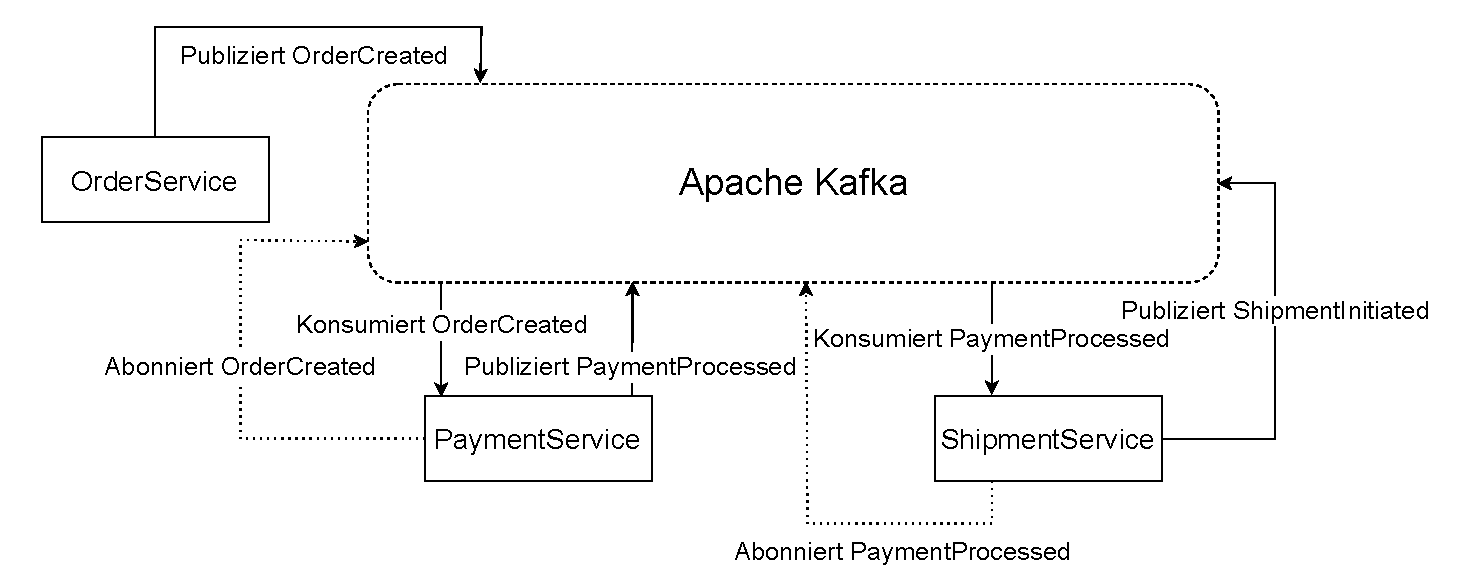
\includegraphics[width=\linewidth]{images/eda/eda-ecommerce.drawio}
  \caption{E-Commerce-Beispiel mit Event-Driven Architecture}
  \label{fig:edaecommerce}
\end{figure}
Wie Abbildung \ref{fig:edaecommerce} zeigt, sind alle drei Dienste Produzenten und Publisher, erzeugen also Events und veröffentlichen diese.
Die Dienste \texttt{PaymentService} und \texttt{ShipmentService} sind zudem Konsumenten,
sodass ersterer auf Events des Typs \texttt{OrderCreated} und zweiterer auf Events des Typs \texttt{ShipmentInitiated} reagiert.
Eine beispielhafte Implementierung des \texttt{PaymentService} mit Apache Kafka als Event-Broker ist im Anhang \ref{app:code:eda:paymentservice} zu finden.
Die vollständige Implementierung des E-Commerce-Beispiels ist bei GitHub \footnote{https://github.com/Beleg-6-EAP/demo-eda-ecommerce} zu finden.

Das Beispiel zeigt, dass die Event-Driven Architektur mit weiteren agilen Strukturen wie Microservices kombiniert werden kann, was die Agilität der Architektur weiter erhöht.
Die damit einhergehende Komplexität stellt teilweise hohe Anforderungen an die Entwickler.
Aufgrund der Asynchronität der Behandlung von Ereignissen ist die Testung des Systems meist schwer und die Fehlerbehandlung essentiell.
Mögliche Problemquellen schließen dabei unter anderem Event-Verlust, erhöhte Latenz und Inkonsistenz ein.
Die hohen Anforderungen an die Entwickler verlangen viel Vertrauen in jene, einer der zentralen Punkte des agilen Manifests \cite{agileManifesto}.
Insgesamt weist die Event-Driven Architecture also eine sehr hohe Agilität auf und ist damit besonders für moderne Software und ihre stetig wechselnden Anforderungen geeignet.

\section{Fallstudien und Praxisbeispiele}
Blah \ldots

\section{Diskussion}

\section{Zusammenfassung und Ausblick}
%(Überblick über die gesamte Arbeit, Rückführung auf Aussagen aus Kapitel 1 durchführen, offene Punkte als neue Forschungsfragen definieren)






\bibliographystyle{ACM-Reference-Format}
\bibliography{main}

\appendix

\section{Code-Beispiele}

\subsection{Event-Driven-Architecture}
\label{app:code:eda:paymentservice}
\begin{listing}[H]
  \tiny
  \inputminted[linenos=true]{java}{code/eda/PaymentService.java}
  \caption{Service-Implementierung des \texttt{PaymentService} in Java Spring Boot 3.4.1 mit Apache Kafka als Event-Broker}
  \label{listing:semigroup}
\end{listing}

\section{Übungsaufgaben}
\subsection{Übungsaufgabe 1 }
Blah \ldots

\end{document}
\endinput
